
\begin{table}
\renewcommand{\arraystretch}{0.7}
 \begin{tabular}{lcccccc}
\hline \hline \\ 
{} & \multicolumn{2}{c}{Maryland} & \multicolumn{2}{c}{North Carolina} & \multicolumn{2}{c}{Pennsylvania} \\
\\ \hline \\
107th Congress         &     0.71 &          \includegraphics[width=6.5em]{splits/md_107} &           0.79 &          \includegraphics[width=6.5em]{splits/nc_107} &         0.87 &          \includegraphics[width=6.5em]{splits/pa_107} \\
111th Congress         &     0.62 &          \includegraphics[width=6.5em]{splits/md_111} &           0.73 &          \includegraphics[width=6.5em]{splits/nc_111} &         0.77 &          \includegraphics[width=6.5em]{splits/pa_111} \\
114th Congress         &     0.58 &          \includegraphics[width=6.5em]{splits/md_114} &           0.71 &          \includegraphics[width=6.5em]{splits/nc_114} &         0.72 &          \includegraphics[width=6.5em]{splits/pa_114} \\
\\ \hline \\ 
Areal Distance         &     0.70 &       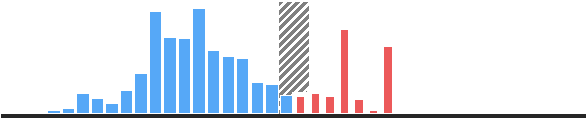
\includegraphics[width=6.5em]{splits/md_dist_a} &           0.78 &       
\includegraphics[width=6.5em]{splits/nc_dist_a} &         0.70 &       \includegraphics[width=6.5em]{splits/pa_dist_a} \\
Axis Ratio             &     0.67 &   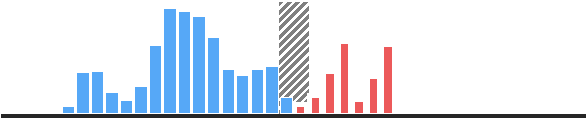
\includegraphics[width=6.5em]{splits/md_axis_ratio} &           0.74 &   
\includegraphics[width=6.5em]{splits/nc_axis_ratio} &         0.69 &   \includegraphics[width=6.5em]{splits/pa_axis_ratio} \\
Circumscribing Circles &     0.68 &        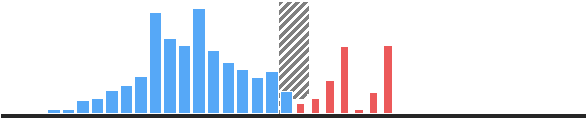
\includegraphics[width=6.5em]{splits/md_reock} &           0.77 &        
\includegraphics[width=6.5em]{splits/nc_reock} &         0.69 &        \includegraphics[width=6.5em]{splits/pa_reock} \\
Distance to Perimeter  &     0.67 &     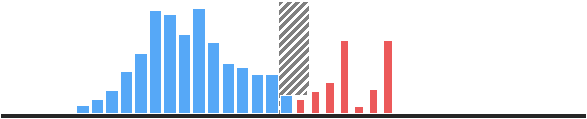
\includegraphics[width=6.5em]{splits/md_rohrbach} &           0.75 &     
\includegraphics[width=6.5em]{splits/nc_rohrbach} &         0.68 &     \includegraphics[width=6.5em]{splits/pa_rohrbach} \\
Dynamic Radius         &     0.69 &   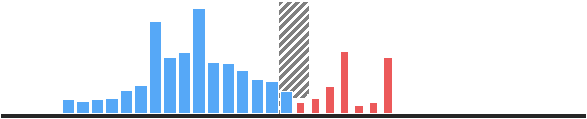
\includegraphics[width=6.5em]{splits/md_dyn_radius} &           0.78 &   
\includegraphics[width=6.5em]{splits/nc_dyn_radius} &         0.71 &   \includegraphics[width=6.5em]{splits/pa_dyn_radius} \\
Exchange               &     0.68 &     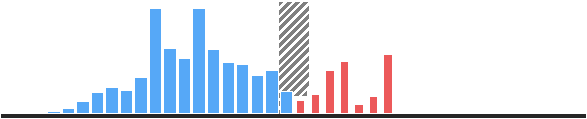
\includegraphics[width=6.5em]{splits/md_exchange} &           0.77 &     
\includegraphics[width=6.5em]{splits/nc_exchange} &         0.70 &     \includegraphics[width=6.5em]{splits/pa_exchange} \\
Harmonic Radius        &     0.68 &  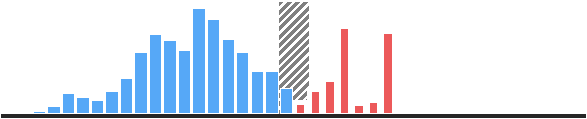
\includegraphics[width=6.5em]{splits/md_harm_radius} &           0.79 &  
\includegraphics[width=6.5em]{splits/nc_harm_radius} &         0.71 &  \includegraphics[width=6.5em]{splits/pa_harm_radius} \\
Hull Area              &     0.68 &       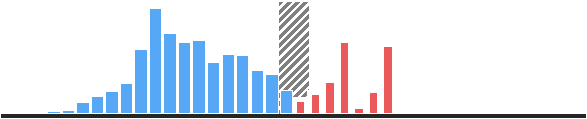
\includegraphics[width=6.5em]{splits/md_hull_a} &           0.76 &       
\includegraphics[width=6.5em]{splits/nc_hull_a} &         0.67 &       \includegraphics[width=6.5em]{splits/pa_hull_a} \\
Hull Population        &     0.66 &       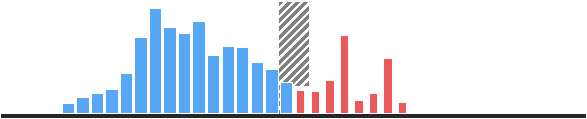
\includegraphics[width=6.5em]{splits/md_hull_p} &           0.74 &       
\includegraphics[width=6.5em]{splits/nc_hull_p} &         0.67 &       \includegraphics[width=6.5em]{splits/pa_hull_p} \\
Inertia Area           &     0.69 &    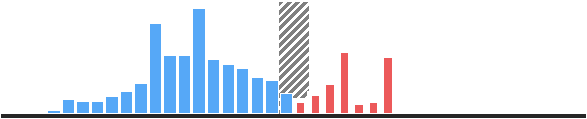
\includegraphics[width=6.5em]{splits/md_inertia_a} &           0.78 &    
\includegraphics[width=6.5em]{splits/nc_inertia_a} &         0.70 &    \includegraphics[width=6.5em]{splits/pa_inertia_a} \\
Inertia Population     &     0.70 &    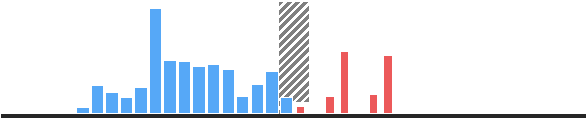
\includegraphics[width=6.5em]{splits/md_inertia_p} &           0.78 &    
\includegraphics[width=6.5em]{splits/nc_inertia_p} &         0.72 &    \includegraphics[width=6.5em]{splits/pa_inertia_p} \\
Inscribed Circles      &     0.67 &    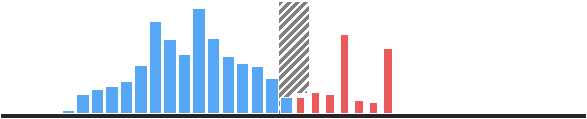
\includegraphics[width=6.5em]{splits/md_ehrenburg} &           0.76 &    
\includegraphics[width=6.5em]{splits/nc_ehrenburg} &         0.69 &    \includegraphics[width=6.5em]{splits/pa_ehrenburg} \\
Isoperimeter Quotient  &     0.66 &       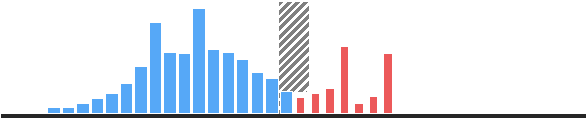
\includegraphics[width=6.5em]{splits/md_polsby} &           0.77 &       
\includegraphics[width=6.5em]{splits/nc_polsby} &         0.69 &       \includegraphics[width=6.5em]{splits/pa_polsby} \\
County-Weighted IPQ    &     0.69 &     \includegraphics[width=6.5em]{splits/md_polsby_w} &           0.81 &     \includegraphics[width=6.5em]{splits/nc_polsby_w} &         0.73 &     \includegraphics[width=6.5em]{splits/pa_polsby_w} \\
Path Fraction          &     0.62 &    \includegraphics[width=6.5em]{splits/md_path_frac} &           0.73 &    \includegraphics[width=6.5em]{splits/nc_path_frac} &         0.64 &    \includegraphics[width=6.5em]{splits/pa_path_frac} \\
Population Distance    &     0.70 &       \includegraphics[width=6.5em]{splits/md_dist_p} &           0.80 &       \includegraphics[width=6.5em]{splits/nc_dist_p} &         0.73 &       \includegraphics[width=6.5em]{splits/pa_dist_p} \\
Power Diagram          &     0.69 &        \includegraphics[width=6.5em]{splits/md_power} &           0.78 &        \includegraphics[width=6.5em]{splits/nc_power} &         0.71 &        \includegraphics[width=6.5em]{splits/pa_power} \\
\raisebox{1.3em}{Split-Line}              &      \raisebox{1.3em}{0.71}  &        \includegraphics[width=6.5em]{splits/md_split_ax} &            \raisebox{1.3em}{0.77}  &        \includegraphics[width=6.5em]{splits/nc_split_ax} &          \raisebox{1.3em}{0.70}  &        \includegraphics[width=6.5em]{splits/pa_split_ax} \\
\hline \hline
\end{tabular}
\caption{
Probability of a citizen of a county living in the same congressional district
  as another randomly-selected citizen of their county, for distributions of maps
  derived for various compactness definitions.
The ``probability" is modified to account for counties larger than
  Congressional Districts (see text).
North Carolina gained a seat after the 2000 Census, 
  whereas Pennsylvania lost seats in both 2002 and 2012.
The probabilities do not not correct for this effect (first three rows).
There is a progression towards more-dividied counties
  among the enacted maps.
For Maryland and North Carolina, the automated procedures 
  outperform the enacted maps.
The county-weighted isoperimeter quotient measure outperforms 
  baseline IPQ by a few percent.
}\label{tab:competitiveness}
\end{table}
 